\documentclass[lualatex,ja=standard,a4paper,12pt]{bxjsarticle}
\usepackage{amsmath, amssymb, amsthm, bm}
\usepackage{geometry}
\usepackage{xcolor}
\usepackage{tcolorbox}
\usepackage{booktabs}
\usepackage{array}
\usepackage{tikz}
\usetikzlibrary{positioning, arrows.meta}
\usepackage{pgfplots}
\pgfplotsset{compat=1.18}

\geometry{margin=25mm}

\tcbuselibrary{theorems, skins, breakable}

\newtcolorbox{defbox}[1]{
  colback=blue!5, colframe=blue!60!black,
  fonttitle=\bfseries, title={#1}, arc=3pt, breakable
}
\newtcolorbox{thmbox}[1]{
  colback=green!5, colframe=green!50!black,
  fonttitle=\bfseries, title={#1}, arc=3pt, breakable
}
\newtcolorbox{pointbox}{
  colback=orange!8, colframe=orange!70!black,
  fonttitle=\bfseries, title={ポイント}, arc=3pt, breakable
}
\newtcolorbox{exbox}[1]{
  colback=gray!6, colframe=gray!50,
  fonttitle=\bfseries, title={例：#1}, arc=3pt, breakable
}
\newtcolorbox{derivbox}{
  colback=purple!4, colframe=purple!50!black,
  fonttitle=\bfseries, title={導出}, arc=3pt, breakable
}
\newtcolorbox{warningbox}{
  colback=red!5, colframe=red!60!black,
  fonttitle=\bfseries, title={注意}, arc=3pt, breakable
}
\newtcolorbox{algobox}[1]{
  colback=cyan!4, colframe=cyan!50!black,
  fonttitle=\bfseries, title={#1}, arc=3pt, breakable
}

\newcommand{\IG}{\mathrm{inverse\text{-}gamma}}

\title{{\large Hoff 第8章} \\[6pt]
       \textbf{Group Comparisons and Hierarchical Modeling} \\[4pt]
       {\normalsize （グループ比較と階層モデル）ゼミ資料}}
\author{}
\date{}

\begin{document}
\maketitle
\thispagestyle{empty}

% ===========================
\section{この章のモチベーション}
% ===========================

この章のテーマは\textbf{複数のグループの平均の比較}である．
\begin{itemize}
  \item \textbf{2グループ}（8.1節）：2つの平均を「平均」と「差」で表し直す．
  \item \textbf{多グループ}（8.2--8.4節）：グループ平均たちの「全体の平均」と「バラつき」も正規分布でモデル化する．
        グループ内のバラつきのモデルと合わせて\textbf{階層正規モデル}になる．
  \item \textbf{分散も階層化}（8.5節）：グループごとに分散も違ってよいように拡張する．
\end{itemize}

\begin{pointbox}
章全体を通じたキーワードは\textbf{「グループ間で情報を共有する」}こと．
「全グループを完全に別物として扱う」と「全グループを同一視する」の両極端の間で，
データに応じて連続的に情報を借りる．その結果として\textbf{縮小推定}（shrinkage）が起こる．
\end{pointbox}

% ===========================
\section{2つのグループの比較（8.1節）}
% ===========================

\subsection{古典的なやり方：$t$ 検定と $p$ 値}

\begin{exbox}{2校の数学の点数}
米国の都市部の公立高校2校から，10年生をそれぞれ $n_1 = 31$ 人，$n_2 = 28$ 人無作為に選んでテストした．
標本平均は $\bar{y}_1 = 50.81$，$\bar{y}_2 = 46.15$ で，差は $4.66$．

\medskip
この差が標本のばらつきに比べて大きいかを見るため，$t$ 統計量を計算すると
\[
  t = \frac{\bar{y}_1 - \bar{y}_2}{s_p\sqrt{1/n_1 + 1/n_2}} = 1.74,
  \qquad
  s_p^2 = \frac{(n_1-1)s_1^2 + (n_2-1)s_2^2}{n_1 + n_2 - 2}.
\]
2校が同じ正規分布なら $t$ は自由度 $57$ の $t$ 分布に従い，両側 $p$ 値は $p = 0.087$．
\end{exbox}

\begin{warningbox}
$p$ 値は「$\theta_1 = \theta_2$ である確率」\textbf{ではない}．
「2校が同じ分布だと仮定したとき，実験前に $|t| \ge 1.74$ となるデータを引く確率」である．
\end{warningbox}

\subsubsection*{$p$ 値によるモデル選択の問題点}

よく教えられる手順は次のとおり：
\begin{itemize}
  \item $p < 0.05$ なら「2校は別物」として $\hat{\theta}_1 = \bar{y}_1$，$\hat{\theta}_2 = \bar{y}_2$．
  \item $p > 0.05$ なら「2校は同じ」として $\hat{\theta}_1 = \hat{\theta}_2 = $ 全員の平均．
\end{itemize}

これは $\hat{\theta}_1 = w\bar{y}_1 + (1-w)\bar{y}_2$ と書いたとき，
\[
  w = 1 \;\;(p < 0.05), \qquad w = \frac{n_1}{n_1 + n_2} \;\;(p > 0.05)
\]
と\textbf{0か1かの極端な切り替え}をしていることになる．

\begin{itemize}
  \item 今回は $p = 0.087$ なので「同じ」扱いになるが，差がありそうな証拠もある．
  \item 逆に，標本にたまたま数人の成績上位者が混ざれば $p = 0.04$ になり，
        今度は2校を完全に別々に推定する．他校のデータを全く使わないのは非効率．
\end{itemize}

\begin{pointbox}
本当は $w$ を\textbf{連続的に}動かし，サンプルサイズ $n_1, n_2$，ばらつき $\sigma^2$，
2校が似ているという事前情報などに応じて決めたい．
グループ間で情報を共有するベイズ解析は，まさにそういう推定量を与える．
\end{pointbox}

\subsection{ベイズモデル：平均と差でパラメータ化する}

\begin{defbox}{2グループのモデル}
\begin{align*}
  Y_{i,1} &= \mu + \delta + \epsilon_{i,1}, \\
  Y_{i,2} &= \mu - \delta + \epsilon_{i,2}, \qquad
  \{\epsilon_{i,j}\} \overset{\text{i.i.d.}}{\sim} \mathrm{Normal}(0, \sigma^2).
\end{align*}
$\theta_1 = \mu + \delta$，$\theta_2 = \mu - \delta$ なので
\[
  \mu = \frac{\theta_1 + \theta_2}{2} \;\;\text{（2校の平均）}, \qquad
  \delta = \frac{\theta_1 - \theta_2}{2} \;\;\text{（差の半分）}.
\]
\textbf{事前分布}（独立）：
$\mu \sim \mathrm{Normal}(\mu_0, \gamma_0^2)$，
$\delta \sim \mathrm{Normal}(\delta_0, \tau_0^2)$，
$\sigma^2 \sim \IG(\nu_0/2,\, \nu_0\sigma_0^2/2)$．
\end{defbox}

\subsubsection*{完全条件付き分布}

\begin{thmbox}{$\mu, \delta, \sigma^2$ の完全条件付き分布}
\begin{align*}
  \{\mu \mid \bm{y}_1, \bm{y}_2, \delta, \sigma^2\} &\sim \mathrm{Normal}(\mu_n, \gamma_n^2), \\
  &\quad \gamma_n^2 = \bigl[1/\gamma_0^2 + (n_1+n_2)/\sigma^2\bigr]^{-1}, \\
  &\quad \mu_n = \gamma_n^2\Bigl[\mu_0/\gamma_0^2 + \textstyle\sum_i (y_{i,1} - \delta)/\sigma^2 + \sum_i (y_{i,2} + \delta)/\sigma^2\Bigr], \\[4pt]
  \{\delta \mid \bm{y}_1, \bm{y}_2, \mu, \sigma^2\} &\sim \mathrm{Normal}(\delta_n, \tau_n^2), \\
  &\quad \tau_n^2 = \bigl[1/\tau_0^2 + (n_1+n_2)/\sigma^2\bigr]^{-1}, \\
  &\quad \delta_n = \tau_n^2\Bigl[\delta_0/\tau_0^2 + \textstyle\sum_i (y_{i,1} - \mu)/\sigma^2 - \sum_i (y_{i,2} - \mu)/\sigma^2\Bigr], \\[4pt]
  \{\sigma^2 \mid \bm{y}_1, \bm{y}_2, \mu, \delta\} &\sim \IG(\nu_n/2,\, \nu_n\sigma_n^2/2), \\
  &\quad \nu_n = \nu_0 + n_1 + n_2, \\
  &\quad \nu_n\sigma_n^2 = \nu_0\sigma_0^2 + \textstyle\sum_i (y_{i,1} - [\mu + \delta])^2 + \sum_i (y_{i,2} - [\mu - \delta])^2.
\end{align*}
\end{thmbox}

\begin{derivbox}
教科書では演習問題になっている．$\delta$ について確かめる．
$\delta$ を含む因子だけを集めると
\[
  p(\delta \mid \cdots) \propto
  \exp\Bigl\{-\tfrac{(\delta - \delta_0)^2}{2\tau_0^2}\Bigr\}
  \prod_i \exp\Bigl\{-\tfrac{(y_{i,1} - \mu - \delta)^2}{2\sigma^2}\Bigr\}
  \prod_i \exp\Bigl\{-\tfrac{(y_{i,2} - \mu + \delta)^2}{2\sigma^2}\Bigr\}.
\]
$z_{i,1} = y_{i,1} - \mu$，$z_{i,2} = -(y_{i,2} - \mu)$ とおくと，どちらも
「$\delta$ を平均とし分散 $\sigma^2$ の正規分布からの観測」と同じ形になる
（$(y_{i,2} - \mu + \delta)^2 = (z_{i,2} - \delta)^2$）．
すると $n_1 + n_2$ 個の観測 $z$ と正規事前分布の組み合わせなので，
5.2節（分散既知の正規モデル）の結果がそのまま使えて，
精度 $1/\tau_n^2 = 1/\tau_0^2 + (n_1+n_2)/\sigma^2$，
平均 $\delta_n = \tau_n^2[\delta_0/\tau_0^2 + \sum z_{i,1}/\sigma^2 + \sum z_{i,2}/\sigma^2]$ を得る．
$\mu$ も同様（$y_{i,1} - \delta$ と $y_{i,2} + \delta$ を「$\mu$ を平均とする観測」とみる）．
\end{derivbox}

\begin{pointbox}
\textbf{極端な値を入れて納得する：}
\begin{itemize}
  \item $\nu_0 = 0$ なら $\sigma_n^2 = \dfrac{\sum(y_{i,1} - [\mu+\delta])^2 + \sum(y_{i,2} - [\mu-\delta])^2}{n_1 + n_2}$
        ——$\mu, \delta$ が既知のときのプールした分散推定量．
  \item $\mu_0 = \delta_0 = 0$，$\gamma_0^2 = \tau_0^2 = \infty$ なら
        $\mu_n = \dfrac{\sum(y_{i,1} - \delta) + \sum(y_{i,2} + \delta)}{n_1 + n_2}$，
        $\delta_n = \dfrac{\sum(y_{i,1} - \mu) - \sum(y_{i,2} - \mu)}{n_1 + n_2}$ で，
        $\mu_n, \delta_n$ を代入し合うと $\bar{y}_1 = \mu_n + \delta_n$，$\bar{y}_2 = \mu_n - \delta_n$．
\end{itemize}
\end{pointbox}

\subsection{数学の点数データの解析}

\subsubsection*{事前分布の設定}
テストは全国平均 $50$，標準偏差 $10$ になるよう標準化されている．
\begin{center}
\renewcommand{\arraystretch}{1.4}
\begin{tabular}{lll}
\toprule
パラメータ & 設定 & 理由 \\
\midrule
$\mu_0, \gamma_0^2$ & $50,\; 25^2 = 625$ & 全国平均．やや拡散的に \\
$\sigma_0^2, \nu_0$ & $10^2 = 100,\; 1$ & 全国の分散（学校内の分散としては過大）．弱く \\
$\delta_0$ & $0$ & $\theta_1 > \theta_2$ と $\theta_2 > \theta_1$ を同程度に信じる \\
$\tau_0^2$ & $25^2 = 625$ & 点数は 0〜100 なので $|\delta| < 50$．十分拡散的 \\
\bottomrule
\end{tabular}
\end{center}

\subsubsection*{結果}

Gibbs サンプラーを 5,000 回まわすと：
\begin{itemize}
  \item $\mu, \delta$ の事後分布は事前分布よりずっと集中する（教科書 Figure 8.2）．
  \item 2校の平均点の差 $2\delta$ の事後 95\% 区間は $(-0.61,\, 9.98)$．0 を含むが，
  \item $\Pr(\theta_1 > \theta_2 \mid \bm{y}_1, \bm{y}_2) = \Pr(\delta > 0 \mid \bm{y}_1, \bm{y}_2) \approx 0.96$
        （事前確率は $0.50$）．学校1の母平均の方が高いという\textbf{かなりの証拠}がある．
\end{itemize}

\begin{warningbox}
$\Pr(\theta_1 > \theta_2 \mid \bm{y}) \approx 0.96$ を
「学校1から無作為に選んだ生徒が学校2の生徒より高得点である確率」と混同しないこと．
後者は\textbf{事後予測分布}から求める量で，$\Pr(\tilde{Y}_1 > \tilde{Y}_2 \mid \bm{y}_1, \bm{y}_2) \approx 0.62$ にすぎない．
「平均の比較」と「個人の比較」は別物である（11章の $\theta_2$ と $\tilde{\beta}_2$ の区別と同じ構造）．
\end{warningbox}

% ===========================
\section{多グループの比較：交換可能性と階層モデル（8.2節）}
% ===========================

\subsection{階層データ（多段階データ）}

8.1節のデータは，2002年の教育縦断調査（ELS）の一部である．
ELS には\textbf{学校の集団}と，\textbf{各学校の中の生徒の集団}がある．
このように集団が入れ子になったデータを\textbf{階層データ}・\textbf{多段階データ}（multilevel）と呼ぶ．
\begin{itemize}
  \item 複数の病院の中の患者
  \item 動物の集団の中の遺伝子
  \item 国の中の地域の中の郡の中の人
\end{itemize}
最も単純な2段階の場合，グループ $j$ の $i$ 番目のデータを $y_{i,j}$ と書く．

\subsection{交換可能性から階層モデルを導く}

\begin{defbox}{交換可能性（第2章の復習）}
$p(y_1, \ldots, y_n) = p(y_{\pi_1}, \ldots, y_{\pi_n})$ が任意の並べ替え $\pi$ について成り立つとき，
$Y_1, \ldots, Y_n$ は\textbf{交換可能}という．
すべての $n$ で交換可能なら，\textbf{de Finetti の定理}により
\[
  \phi \sim p(\phi), \qquad \{Y_1, \ldots, Y_n \mid \phi\} \overset{\text{i.i.d.}}{\sim} p(y \mid \phi)
\]
と表せる（固定だが未知の母集団の特徴 $\phi$ を条件とした i.i.d. 標本）．
\end{defbox}

\noindent この定理を\textbf{2回}使う：

\begin{enumerate}
  \item \textbf{グループ内}：同じ学校の生徒の点数は，互いに独立とは扱いたくない
        （他の生徒の点数から，その学校の水準について情報が得られるはず）．
        しかし「学校 $j$ からの無作為標本」以上の情報がなければ\textbf{交換可能}とみなせる．
        $\Rightarrow$ $\{Y_{1,j}, \ldots, Y_{n_j,j} \mid \phi_j\} \overset{\text{i.i.d.}}{\sim} p(y \mid \phi_j)$．
  \item \textbf{グループ間}：学校ごとのパラメータ $\phi_1, \ldots, \phi_m$ も独立とは扱いたくない
        （他校の値から $\phi_m$ について情報が得られるはず）．
        しかし学校自体がより大きな学校の集団からの標本なら，\textbf{交換可能}とみなせる．
        $\Rightarrow$ $\{\phi_1, \ldots, \phi_m \mid \psi\} \overset{\text{i.i.d.}}{\sim} p(\phi \mid \psi)$．
\end{enumerate}

\begin{thmbox}{階層モデルの3つの分布}
\begin{align*}
  \{y_{1,j}, \ldots, y_{n_j,j} \mid \phi_j\} &\overset{\text{i.i.d.}}{\sim} p(y \mid \phi_j) && \text{（グループ内の標本変動）} \\
  \{\phi_1, \ldots, \phi_m \mid \psi\} &\overset{\text{i.i.d.}}{\sim} p(\phi \mid \psi) && \text{（グループ間の標本変動）} \\
  \psi &\sim p(\psi) && \text{（事前分布）}
\end{align*}
\end{thmbox}

\begin{warningbox}
$p(y \mid \phi)$ と $p(\phi \mid \psi)$ はどちらも\textbf{対象の集団の中でのばらつき}を表す
\textbf{標本抽出分布}である（前者は生徒間，後者は学校間）．
一方 $p(\psi)$ は\textbf{固定された未知量についての情報}を表す\textbf{事前分布}．
データから推定されるのは $p(y \mid \phi)$ と $p(\phi \mid \psi)$ のほうで，$p(\psi)$ はデータから推定しない．
$p(\phi \mid \psi)$ を「事前分布」と呼ぶ文献も多いが，概念的には区別すべきである．
\end{warningbox}

% ===========================
\section{階層正規モデル（8.3節）}
% ===========================

\begin{defbox}{階層正規モデル}
\begin{align*}
  \phi_j = \{\theta_j, \sigma^2\},\quad & p(y \mid \phi_j) = \mathrm{Normal}(\theta_j, \sigma^2) && \text{（グループ内モデル）} \tag{8.1} \\
  \psi = \{\mu, \tau^2\},\quad & p(\theta_j \mid \psi) = \mathrm{Normal}(\mu, \tau^2) && \text{（グループ間モデル）} \tag{8.2}
\end{align*}
\textbf{事前分布}（半共役）：
\begin{align*}
  1/\sigma^2 &\sim \mathrm{gamma}(\nu_0/2,\, \nu_0\sigma_0^2/2), \\
  1/\tau^2 &\sim \mathrm{gamma}(\eta_0/2,\, \eta_0\tau_0^2/2), \\
  \mu &\sim \mathrm{Normal}(\mu_0, \gamma_0^2).
\end{align*}
\end{defbox}

\noindent グループ内の分散 $\sigma^2$ は\textbf{全グループ共通}と仮定している（8.5節で外す）．

\begin{center}
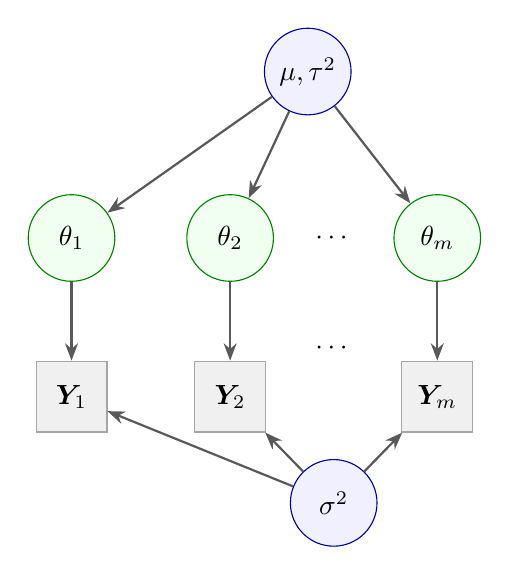
\begin{tikzpicture}[
  node distance=10mm and 9mm,
  param/.style={circle, draw=blue!60!black, fill=blue!6, minimum size=11mm, inner sep=1pt},
  grp/.style={circle, draw=green!50!black, fill=green!6, minimum size=11mm, inner sep=1pt},
  obs/.style={rectangle, draw=gray!70, fill=gray!12, minimum size=9mm, inner sep=2pt},
  arr/.style={-{Stealth[length=2.2mm]}, thick, gray!70!black}
]
  \node[param] (mt) {$\mu, \tau^2$};
  \node[grp, below=of mt, xshift=-30mm] (t1) {$\theta_1$};
  \node[grp, right=of t1] (t2) {$\theta_2$};
  \node[right=4mm of t2] (td) {$\cdots$};
  \node[grp, right=4mm of td] (tm) {$\theta_m$};
  \node[obs, below=of t1] (y1) {$\bm{Y}_1$};
  \node[obs, below=of t2] (y2) {$\bm{Y}_2$};
  \node[below=10mm of td] (yd) {$\cdots$};
  \node[obs, below=of tm] (ym) {$\bm{Y}_m$};
  \node[param, below=12mm of yd] (s2) {$\sigma^2$};
  \foreach \t in {t1,t2,tm} \draw[arr] (mt) -- (\t);
  \draw[arr] (t1) -- (y1); \draw[arr] (t2) -- (y2); \draw[arr] (tm) -- (ym);
  \foreach \y in {y1,y2,ym} \draw[arr] (s2) -- (\y);
\end{tikzpicture}

\smallskip
{\small 図1：階層正規モデルのグラフ表現（教科書 Figure 8.3）．
青：全体のパラメータ，緑：グループ固有のパラメータ，灰：観測データ．}
\end{center}

\subsection{事後分布の分解}

同時事後分布は次のように分解できる：
\begin{align*}
  p(\theta_1, \ldots, \theta_m, \mu, \tau^2, \sigma^2 \mid \bm{y}_1, \ldots, \bm{y}_m)
  &\propto p(\mu)\,p(\tau^2)\,p(\sigma^2)
   \;\times\; \Bigl\{\prod_{j=1}^m p(\theta_j \mid \mu, \tau^2)\Bigr\} \\
  &\qquad \times\; \Bigl\{\prod_{j=1}^m \prod_{i=1}^{n_j} p(y_{i,j} \mid \theta_j, \sigma^2)\Bigr\}. \tag{8.3}
\end{align*}
最後の括弧は\textbf{条件付き独立性}による：$\theta_j, \sigma^2$ が与えられれば
$Y_{1,j}, \ldots, Y_{n_j,j}$ は独立で，$\mu, \tau^2$ には依存しない．
図1で $(\mu, \tau^2)$ から $\bm{Y}_j$ への経路は必ず $\theta_j$ を通る
——$(\mu, \tau^2)$ は $\bm{Y}_j$ に\textbf{$\theta_j$ を通じて間接的にしか}影響しない．

\begin{pointbox}
完全条件付き分布は，(8.3) から\textbf{そのパラメータを含む因子だけを拾えば}求まる．
そして拾った因子は，どれも第5・6章の「1標本の正規モデル」と全く同じ形をしている．
新しい計算はほとんど要らず，\textbf{記号の読み替え}だけで済む．
\end{pointbox}

\subsection{完全条件付き分布（8.3.1節）}

\begin{center}
\small
\renewcommand{\arraystretch}{1.5}
\setlength{\tabcolsep}{4pt}
\begin{tabular}{llll}
\toprule
パラメータ & (8.3) から拾う因子 & 第6章での対応 & 分布 \\
\midrule
$\mu$ & $p(\mu)\prod_j p(\theta_j \mid \mu, \tau^2)$ & $\theta_j$ をデータ，$\mu$ を母平均とみる & 正規 \\
$\tau^2$ & $p(\tau^2)\prod_j p(\theta_j \mid \mu, \tau^2)$ & $\theta_j$ をデータ，$\tau^2$ を母分散とみる & 逆ガンマ \\
$\theta_j$ & $p(\theta_j \mid \mu, \tau^2)\prod_i p(y_{i,j} \mid \theta_j, \sigma^2)$ & $p(\theta_j \mid \mu, \tau^2)$ を事前分布とみる & 正規 \\
$\sigma^2$ & $p(\sigma^2)\prod_j\prod_i p(y_{i,j} \mid \theta_j, \sigma^2)$ & $m$ グループ分の残差を使う & 逆ガンマ \\
\bottomrule
\end{tabular}
\end{center}

\begin{thmbox}{$\mu$ と $\tau^2$ の完全条件付き分布}
\begin{align*}
  \{\mu \mid \theta_1, \ldots, \theta_m, \tau^2\} &\sim
    \mathrm{Normal}\!\left(\frac{m\bar{\theta}/\tau^2 + \mu_0/\gamma_0^2}{m/\tau^2 + 1/\gamma_0^2},\;
    \bigl[m/\tau^2 + 1/\gamma_0^2\bigr]^{-1}\right), \\
  \{1/\tau^2 \mid \theta_1, \ldots, \theta_m, \mu\} &\sim
    \mathrm{gamma}\!\left(\frac{\eta_0 + m}{2},\; \frac{\eta_0\tau_0^2 + \sum_j (\theta_j - \mu)^2}{2}\right).
\end{align*}
\end{thmbox}

\noindent $\theta_1, \ldots, \theta_m$ が「正規母集団からの i.i.d. 標本」，$\mu, \tau^2$ が「その母平均・母分散」
という第6章と全く同じ状況なので，結果も記号を読み替えただけである．

\begin{thmbox}{$\theta_j$ の完全条件付き分布}
\[
  \{\theta_j \mid y_{1,j}, \ldots, y_{n_j,j}, \mu, \tau^2, \sigma^2\} \sim
  \mathrm{Normal}\!\left(\frac{n_j\bar{y}_j/\sigma^2 + \mu/\tau^2}{n_j/\sigma^2 + 1/\tau^2},\;
  \bigl[n_j/\sigma^2 + 1/\tau^2\bigr]^{-1}\right).
\]
\end{thmbox}

\noindent $\mu, \tau^2, \sigma^2, \bm{y}_j$ を条件にすると，$\theta_j$ は他の $\theta_k$ や他グループのデータと\textbf{独立}．
図1で $\theta_j$ から $\theta_k$ への経路は必ず $(\mu, \tau^2)$ か $\sigma^2$ を通るためである．
数学的には，$p(\theta_j \mid \mu, \tau^2)$ を「事前分布」とみた1標本の正規モデル（5.2節）と同じ．

\begin{thmbox}{$\sigma^2$ の完全条件付き分布}
\[
  \{1/\sigma^2 \mid \bm{\theta}, \bm{y}_1, \ldots, \bm{y}_m\} \sim
  \mathrm{gamma}\!\left(\frac{\nu_0 + \sum_j n_j}{2},\;
  \frac{\nu_0\sigma_0^2 + \mathrm{SSR}}{2}\right),
\]
ただし $\mathrm{SSR} = \sum_{j=1}^m\sum_{i=1}^{n_j}(y_{i,j} - \theta_j)^2$．
\end{thmbox}

\noindent $\sum\sum(y_{i,j} - \theta_j)^2$ は全グループの残差平方和なので，
この分布は\textbf{プールした分散推定値}のまわりに集中する．

% ===========================
\section{例：米国の公立高校の数学の点数（8.4節）}
% ===========================

\subsection{データの特徴}

ELS の 100 校（いずれも10年生が 400 人以上の都市部の大規模公立高校）のデータ．
学校ごとの標本平均は最低 36.6，最高 65.0 と幅が大きい．

\begin{exbox}{極端な平均はサンプルの少ない学校から出る}
標本平均とサンプルサイズの関係を見ると（教科書 Figure 8.5），
\textbf{極端な標本平均の学校はサンプルサイズが小さい}傾向がある
（平均が最高の学校はサンプルサイズが最小）．

\medskip
\noindent\textbf{理由：}仮に全校の真の平均が同じ $\theta_0$ でも，
\[
  E[\bar{Y}_j \mid \theta_0, \sigma^2] = \theta_0, \qquad
  \mathrm{Var}[\bar{Y}_j \mid \sigma^2] = \sigma^2/n_j
\]
なので，$n_j$ が小さい学校ほど $\bar{y}_j$ が $\theta_0$ から上にも下にも大きく外れやすい．
階層データではよくある現象である．
\end{exbox}

\subsection{事前分布と Gibbs サンプラー（8.4.1節）}

\begin{center}
\renewcommand{\arraystretch}{1.4}
\begin{tabular}{lll}
\toprule
パラメータ & 設定 & 理由 \\
\midrule
$\sigma_0^2, \nu_0$ & $100,\; 1$ & 全国の分散 100 は学校内＋学校間なので，学校内は高々 100 \\
$\tau_0^2, \eta_0$ & $100,\; 1$ & 学校間の分散も 100 を超えないはず \\
$\mu_0, \gamma_0^2$ & $50,\; 25$ & $\mu \in (40, 60)$ の事前確率が約 95\% \\
\bottomrule
\end{tabular}
\end{center}

\begin{algobox}{Gibbs サンプラー（階層正規モデル）}
現在値 $\{\theta_1^{(s)}, \ldots, \theta_m^{(s)}, \mu^{(s)}, \tau^{2(s)}, \sigma^{2(s)}\}$ から：
\begin{enumerate}
  \item $\mu^{(s+1)} \sim p(\mu \mid \theta_1^{(s)}, \ldots, \theta_m^{(s)}, \tau^{2(s)})$
  \item $\tau^{2(s+1)} \sim p(\tau^2 \mid \theta_1^{(s)}, \ldots, \theta_m^{(s)}, \mu^{(s+1)})$
  \item $\sigma^{2(s+1)} \sim p(\sigma^2 \mid \theta_1^{(s)}, \ldots, \theta_m^{(s)}, \bm{y}_1, \ldots, \bm{y}_m)$
  \item 各 $j$ について $\theta_j^{(s+1)} \sim p(\theta_j \mid \mu^{(s+1)}, \tau^{2(s+1)}, \sigma^{2(s+1)}, \bm{y}_j)$
\end{enumerate}
更新の\textbf{順番はどうでもよい}．大事なのは，各パラメータを他のパラメータの\textbf{最新の値}で条件付けて更新すること．
\end{algobox}

\subsubsection*{MCMC の診断}

\begin{itemize}
  \item \textbf{定常性}：サンプル列を 10 等分して箱ひげ図を並べる（教科書 Figure 8.6）．
        定常なら各区間の分布は同じはず．中央値や四分位範囲が一方向に動いていれば，もっと長く回す必要がある．
        今回は問題なし．
  \item \textbf{混ざり具合}：
\end{itemize}

\begin{center}
\renewcommand{\arraystretch}{1.4}
\begin{tabular}{lccc}
\toprule
 & $\mu$ & $\sigma^2$ & $\tau^2$ \\
\midrule
lag-1 自己相関 & 0.15 & 0.053 & 0.312 \\
有効サンプルサイズ & 3706 & 4499 & 2503 \\
モンテカルロ標準誤差 & 0.009 & 0.04 & 0.09 \\
事後平均 & 48.12 & 84.85 & 24.84 \\
\bottomrule
\end{tabular}
\end{center}

\noindent モンテカルロ標準誤差（事後標準偏差 $/\sqrt{\text{有効サンプルサイズ}}$）は事後平均の大きさに比べて十分小さい．
$\theta_j$ たちの有効サンプルサイズは 3,627〜5,927，モンテカルロ標準誤差は 0.02〜0.05．

\subsection{事後要約と縮小推定（8.4.2節）}

$\mu, \sigma, \tau$ の事後平均は $48.12$，$9.21$，$4.97$．したがって
\begin{itemize}
  \item 学校\textbf{内}の点数の約 95\% は互いに $4 \times 9.21 \approx 37$ 点以内，
  \item 学校\textbf{平均}の約 95\% は互いに $4 \times 4.97 \approx 20$ 点以内．
\end{itemize}

\begin{defbox}{縮小（shrinkage）}
$\mu, \tau^2, \sigma^2$ とデータを条件とした $\theta_j$ の期待値は，$\bar{y}_j$ と $\mu$ の加重平均：
\[
  E[\theta_j \mid \bm{y}_j, \mu, \tau, \sigma]
  = \frac{\bar{y}_j\, n_j/\sigma^2 + \mu/\tau^2}{n_j/\sigma^2 + 1/\tau^2}
  = w_j\,\bar{y}_j + (1 - w_j)\,\mu,
  \qquad w_j = \frac{n_j}{n_j + \sigma^2/\tau^2}.
\]
$\theta_j$ の推定値が $\bar{y}_j$ から $\mu$ の方へ $n_j$ に応じた分だけ引き寄せられる．これを\textbf{縮小}と呼ぶ．
\end{defbox}

\noindent 事後平均 $\sigma^2 \approx 84.85$，$\tau^2 \approx 24.84$ を代入すると $\sigma^2/\tau^2 \approx 3.42$ で，
$\bar{y}_j$ にかかる重み $w_j$ はサンプルサイズとともに次のように変わる
（パラメータの不確かさを無視した近似）：

\begin{center}
\begin{tikzpicture}
\begin{axis}[
  width=10cm, height=5.6cm,
  xlabel={サンプルサイズ $n_j$}, ylabel={$\bar{y}_j$ への重み $w_j$},
  xmin=0, xmax=35, ymin=0, ymax=1.05,
  grid=major, grid style={dotted, gray!50},
  tick label style={font=\small}, label style={font=\small},
]
\addplot[blue!70!black, very thick, domain=0.5:35, samples=150] {x/(x+3.416)};
\addplot[only marks, mark=*, mark size=2.2pt, red!70!black] coordinates {(5,0.594) (21,0.860)};
\node[font=\small, anchor=west, red!70!black] at (axis cs:6,0.53) {学校82（$n=5$）：$w \approx 0.59$};
\node[font=\small, anchor=north, red!70!black] at (axis cs:21,0.80) {学校46（$n=21$）：$w \approx 0.86$};
\end{axis}
\end{tikzpicture}

{\small 図2：$w_j = n_j/(n_j + \sigma^2/\tau^2)$，$\sigma^2/\tau^2 = 84.85/24.84 \approx 3.42$．}
\end{center}

\begin{itemize}
  \item $\bar{y}_j$ と $\hat{\theta}_j = E[\theta_j \mid \bm{y}_1, \ldots, \bm{y}_m]$ の関係は，
        \textbf{傾きが1より小さい直線}にほぼ乗る（高い $\bar{y}_j$ は少し低く，低い $\bar{y}_j$ は少し高く推定される）．
  \item \textbf{サンプルの少ない学校ほど強く縮小}され，多い学校はほとんど縮小されない（教科書 Figure 8.8）．
        自分のデータが多ければ，他校から「借りる」情報は少なくて済む．
\end{itemize}

\subsection{順位の逆転：学校46と学校82}

\begin{exbox}{どちらの学校が低いか}
どちらも標本平均が下位 10\% の学校である．

\begin{center}
\renewcommand{\arraystretch}{1.4}
\begin{tabular}{lccc}
\toprule
 & サンプルサイズ & 標本平均 $\bar{y}_j$ & 事後平均 $E[\theta_j \mid \bm{y}]$ \\
\midrule
学校46 & 21 & 40.18 & 41.31 \\
学校82 & 5 & 38.76 & 42.53 \\
\bottomrule
\end{tabular}
\end{center}

標本平均では学校82の方が低いのに，\textbf{事後平均では学校82の方が高い}．順位が逆転している．

\medskip
\noindent\textbf{図2の重みで確かめる：}$E[\mu \mid \bm{y}] \approx 48.11$ として
\begin{align*}
  \text{学校82：} &\; 0.594 \times 38.76 + 0.406 \times 48.11 \approx 42.6, \\
  \text{学校46：} &\; 0.860 \times 40.18 + 0.140 \times 48.11 \approx 41.3,
\end{align*}
と教科書の事後平均をほぼ再現できる．サンプルの少ない学校82の方が，全体平均へ大きく引き寄せられている．
\end{exbox}

\noindent\textbf{なぜこれが妥当か：}
\begin{itemize}
  \item 学校82で最低点の生徒が欠席していたら，$\bar{y}_{82}$ は $38.76 \to 41.99$ と 3 点以上変わる．
  \item 学校46で同じことが起きても，$\bar{y}_{46}$ は $40.18 \to 40.9$ と 0.75 点程度しか変わらない．
  \item つまり学校82の低い平均は「本当に $\theta_{82}$ が低い」とも「たまたま5人のうち数人が成績下位だった」とも説明できるが，
        学校46ではサンプルが多いので後者では説明しにくい．
\end{itemize}

\begin{pointbox}
「学校46の生徒の方が平均点は高かったのに，順位が下なのは不公平」と感じるかもしれない．
しかし階層モデルは「$\theta_{46}$ が極端に低いという\textbf{証拠の量}の方が，$\theta_{82}$ についての証拠より多い」
という客観的事実を反映している．

\medskip
\textbf{バスケットボールの例：}フリースローを3本中3本決めた控え選手（成功率 100\%）と，
成功率 87\% のベテランがいれば，コーチは必ずベテランを選ぶ．
控え選手の真の成功率が 100\% 近いとは考えにくいからである．
\end{pointbox}

% ===========================
\section{平均と分散の両方の階層モデル（8.5節）}
% ===========================

\subsection{グループごとの分散を許す}

平均がグループごとに違うなら，分散も違ってよいはず．
グループ $j$ の分散を $\sigma_j^2$ として $Y_{1,j}, \ldots, Y_{n_j,j} \overset{\text{i.i.d.}}{\sim} \mathrm{Normal}(\theta_j, \sigma_j^2)$ とすると，
$\theta_j$ の完全条件付き分布は $\sigma^2$ を $\sigma_j^2$ に置き換えるだけ：
\[
  \{\theta_j \mid \bm{y}_j, \sigma_j^2, \mu, \tau^2\} \sim
  \mathrm{Normal}\!\left(\frac{n_j\bar{y}_j/\sigma_j^2 + \mu/\tau^2}{n_j/\sigma_j^2 + 1/\tau^2},\;
  \bigl[n_j/\sigma_j^2 + 1/\tau^2\bigr]^{-1}\right).
\]

$\sigma_j^2$ のモデルとして
\[
  1/\sigma_1^2, \ldots, 1/\sigma_m^2 \overset{\text{i.i.d.}}{\sim} \mathrm{gamma}(\nu_0/2,\, \nu_0\sigma_0^2/2) \tag{8.4}
\]
とすれば，第6章と同様に
\[
  \{1/\sigma_j^2 \mid \bm{y}_j, \theta_j\} \sim
  \mathrm{gamma}\!\left(\frac{\nu_0 + n_j}{2},\; \frac{\nu_0\sigma_0^2 + \sum_i (y_{i,j} - \theta_j)^2}{2}\right).
\]

\begin{pointbox}
\textbf{$\nu_0, \sigma_0^2$ を固定すると何がまずいか：}
(8.4) はただの事前分布になり，$p(\sigma_m^2 \mid \sigma_1^2, \ldots, \sigma_{m-1}^2) = p(\sigma_m^2)$．
つまり他の学校の分散から学んだことが $\sigma_m^2$ の推定に使われない．
グループ $m$ のサンプルが少なく，他の $\sigma_j^2$ がある値の周りに集中していれば，その情報を使いたい．

\medskip
$\Rightarrow$ \textbf{$\nu_0, \sigma_0^2$ も推定するパラメータにする}．
すると (8.4) は事前分布ではなく，\textbf{分散の学校間のばらつきを表す標本抽出モデル}になる
（平均における $\mu, \tau^2$ と同じ役割）．
\end{pointbox}

\begin{center}
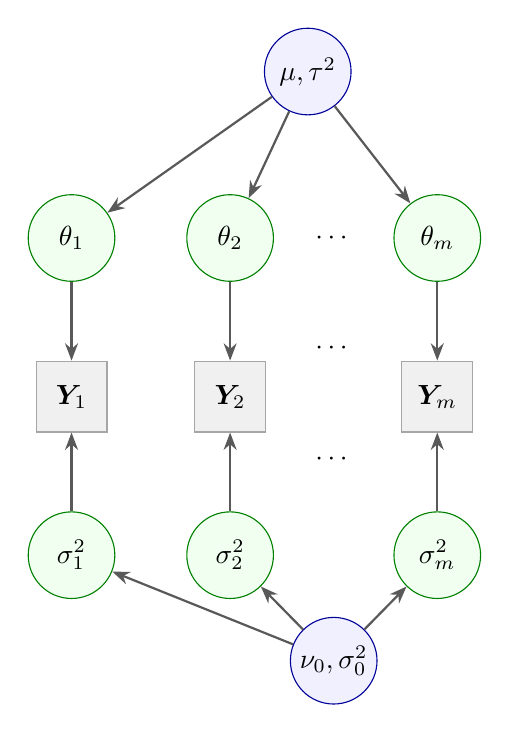
\begin{tikzpicture}[
  node distance=10mm and 9mm,
  param/.style={circle, draw=blue!60!black, fill=blue!6, minimum size=11mm, inner sep=1pt},
  grp/.style={circle, draw=green!50!black, fill=green!6, minimum size=11mm, inner sep=1pt},
  obs/.style={rectangle, draw=gray!70, fill=gray!12, minimum size=9mm, inner sep=2pt},
  arr/.style={-{Stealth[length=2.2mm]}, thick, gray!70!black}
]
  \node[param] (mt) {$\mu, \tau^2$};
  \node[grp, below=of mt, xshift=-30mm] (t1) {$\theta_1$};
  \node[grp, right=of t1] (t2) {$\theta_2$};
  \node[right=4mm of t2] (td) {$\cdots$};
  \node[grp, right=4mm of td] (tm) {$\theta_m$};
  \node[obs, below=of t1] (y1) {$\bm{Y}_1$};
  \node[obs, below=of t2] (y2) {$\bm{Y}_2$};
  \node[below=10mm of td] (yd) {$\cdots$};
  \node[obs, below=of tm] (ym) {$\bm{Y}_m$};
  \node[grp, below=of y1] (s1) {$\sigma_1^2$};
  \node[grp, below=of y2] (s2) {$\sigma_2^2$};
  \node[below=10mm of yd] (sd) {$\cdots$};
  \node[grp, below=of ym] (sm) {$\sigma_m^2$};
  \node[param, below=18mm of sd] (ns) {$\nu_0, \sigma_0^2$};
  \foreach \t in {t1,t2,tm} \draw[arr] (mt) -- (\t);
  \draw[arr] (t1) -- (y1); \draw[arr] (t2) -- (y2); \draw[arr] (tm) -- (ym);
  \draw[arr] (s1) -- (y1); \draw[arr] (s2) -- (y2); \draw[arr] (sm) -- (ym);
  \foreach \s in {s1,s2,sm} \draw[arr] (ns) -- (\s);
\end{tikzpicture}

\smallskip
{\small 図3：平均と分散の両方が異質な階層正規モデル（教科書 Figure 8.10）．}
\end{center}

\subsection{$\nu_0$ と $\sigma_0^2$ の完全条件付き分布}

$\mu, \tau^2$ の完全条件付き分布は前節と変わらない．新たに必要なのは $\sigma_0^2$ と $\nu_0$．

\begin{thmbox}{$\sigma_0^2$ の完全条件付き分布}
事前分布 $\sigma_0^2 \sim \mathrm{gamma}(a, b)$ のもとで
\[
  \{\sigma_0^2 \mid \sigma_1^2, \ldots, \sigma_m^2, \nu_0\} \sim
  \mathrm{gamma}\!\left(a + \frac12 m\nu_0,\;\; b + \frac12\nu_0\sum_{j=1}^m \frac{1}{\sigma_j^2}\right).
\]
\end{thmbox}

\begin{derivbox}
(8.4) の gamma 密度を $\sigma_0^2$ の関数として見ると，各 $j$ について
$\bigl(\nu_0\sigma_0^2/2\bigr)^{\nu_0/2}\exp\{-\tfrac{\nu_0\sigma_0^2}{2}\cdot\tfrac{1}{\sigma_j^2}\}
\propto (\sigma_0^2)^{\nu_0/2}\exp\{-\sigma_0^2 \cdot \tfrac{\nu_0}{2\sigma_j^2}\}$．
$m$ 個かけて事前分布 $(\sigma_0^2)^{a-1}e^{-b\sigma_0^2}$ をかけると
\[
  (\sigma_0^2)^{a + m\nu_0/2 - 1}\exp\Bigl\{-\sigma_0^2\Bigl(b + \tfrac{\nu_0}{2}\textstyle\sum_j 1/\sigma_j^2\Bigr)\Bigr\},
\]
これは上の gamma 分布の核である．
\end{derivbox}

\noindent $a, b$ が小さいとき，条件付き平均 $\approx m / \sum_j (1/\sigma_j^2)$，
つまり $\sigma_1^2, \ldots, \sigma_m^2$ の\textbf{調和平均}になる．

\subsubsection*{$\nu_0$ の完全条件付き分布}

$\nu_0$ には簡単な共役事前分布がない．そこで\textbf{$\nu_0$ を正の整数に制限}し，
幾何分布 $p(\nu_0) \propto e^{-\alpha\nu_0}$（$\nu_0 = 1, 2, \ldots$）を事前分布にすると
\[
  p(\nu_0 \mid \sigma_0^2, \sigma_1^2, \ldots, \sigma_m^2) \propto
  \left(\frac{(\nu_0\sigma_0^2/2)^{\nu_0/2}}{\Gamma(\nu_0/2)}\right)^{\!m}
  \left(\prod_{j=1}^m \frac{1}{\sigma_j^2}\right)^{\!\nu_0/2 - 1}
  \exp\Bigl\{-\nu_0\Bigl(\alpha + \frac12\sigma_0^2\sum_j \frac{1}{\sigma_j^2}\Bigr)\Bigr\}.
\]

\begin{pointbox}
きれいな分布ではないが，$\nu_0 = 1, 2, \ldots, \nu_{\max}$ の各値でこの（正規化されていない）確率を計算し，
その比率で1つ選べばサンプリングできる（\textbf{離散近似}，6.2節と同じ発想）．
数値的には対数で計算し，最大値を引いてから指数をとるとオーバーフローしない．
\end{pointbox}

\subsection{数学の点数データの再解析（8.5.1節）}

事前分布は前節と同じ設定に加えて $\alpha = 1$，$a = 1$，$b = 100$．
Gibbs サンプラーを 5,000 回まわす．

\begin{center}
\renewcommand{\arraystretch}{1.5}
\begin{tabular}{ll}
\toprule
$\nu_0$ の値 & 意味 \\
\midrule
$\nu_0 = \infty$ & 全グループの分散が等しい（8.3節のモデル） \\
$\nu_0 = 1$ & 分散はバラバラで，ほとんど情報を共有しない \\
\textbf{事後：14〜15 付近に集中} & \textbf{どちらの極端でもない，中程度の共有} \\
\bottomrule
\end{tabular}
\end{center}

\noindent 推定された $\sigma_1^2, \ldots, \sigma_m^2$ の分布を使って，極端な標本分散がグループ間の中心に向かって縮小される．
平均のときと同様，\textbf{サンプルの少ない学校ほど分散も強く縮小}される（教科書 Figure 8.12）．

% ===========================
\section{議論と文献（8.6節）}
% ===========================

\begin{itemize}
  \item ベイズ階層モデルの基礎は Lindley and Smith (1972)．
        グループ平均を全体平均へ縮小する発想は，教育テストの文脈で Kelley (1927) にさかのぼる．
  \item 統計学では，この種の推定の利点は\textbf{Stein 効果}（Stein, 1956, 1981）と呼ばれる．
        推定量は一般に $\hat{\theta}_j = w_j\bar{y}_j + (1 - w_j)\bar{y}$ の形で，$w_j$ は $n_j, \sigma^2, \tau^2$ に依存する．
  \item \textbf{経験ベイズ}：$\sigma^2, \tau^2$ をデータから推定して $\hat{\theta}_j$ の式に代入する方法（Efron and Morris, 1973）．
        ベイズとほぼ同じ推定値を与えるが，\textbf{$\sigma^2, \tau^2$ の不確かさを無視している}．
\end{itemize}

\begin{warningbox}
\textbf{用語の混乱：}$y_{i,j} = \theta_j + \epsilon_{i,j}$，$\theta_j = \mu + \gamma_j$ という単純な階層モデルでも，
$\theta_j$（や $\gamma_j$）は推定法によって「固定効果」とも「変量効果」とも呼ばれる．
また $\theta_j$ の分布がしばしば「事前分布」と呼ばれるが，これは事前情報と母集団分布の区別をあいまいにする
（Gelman and Hill, 2007）．

\medskip
\textbf{分散の階層化：}あまり一般的ではないが，グループ内分散が共通だと誤って仮定すると，
不適切な情報のプールや，不適切な量の縮小につながりうる．
\end{warningbox}

% ===========================
\section{まとめ}
% ===========================

\begin{thmbox}{第8章のまとめ}
\begin{enumerate}
  \item $p$ 値によるモデル選択は「完全に別物」か「完全に同じ」かの\textbf{両極端}しか選べない．
        ベイズ解析ではグループ間で\textbf{連続的に}情報を共有できる．

  \item 2グループは $\theta_1 = \mu + \delta$，$\theta_2 = \mu - \delta$ とパラメータ化し，Gibbs で推定する．
        「平均の比較 $\Pr(\theta_1 > \theta_2)$」と「個人の比較 $\Pr(\tilde{Y}_1 > \tilde{Y}_2)$」は別物．

  \item de Finetti の定理を\textbf{グループ内とグループ間の2回}使うと，階層モデル
        （グループ内の標本抽出モデル，グループ間の標本抽出モデル，事前分布）が導かれる．

  \item \textbf{階層正規モデル}の完全条件付き分布は，どれも第5・6章の1標本正規モデルの\textbf{記号の読み替え}で得られる．

  \item 推定値は $\bar{y}_j$ から全体平均 $\mu$ の方へ縮小される．
        重み $w_j = n_j/(n_j + \sigma^2/\tau^2)$ より，\textbf{サンプルの少ないグループほど強く縮小}される．
        その結果，標本平均と事後平均で順位が逆転することもある（学校46と82）．

  \item 分散もグループごとに変えて $\nu_0, \sigma_0^2$ を推定すれば，分散についても情報を共有し縮小できる．
        数学の点数では $\nu_0 \approx 14$〜$15$ で，「全部同じ」と「全部バラバラ」の中間．

  \item この章の階層モデルは，第11章で「平均」を「回帰係数」に一般化した\textbf{階層回帰モデル}へ拡張される．
\end{enumerate}
\end{thmbox}

\end{document}
